\section{Results}

We evaluate the proposed method on the MIMIC dataset by comparing the classification quality of the MoPoE to supervised classification methods in a first step and then evaluate the generation quality and coherence in a second step.
In the following section, we will abbreviate the three modalities present in the data selection with "F" for frontal scan, "L" for lateral scan and "T" for text report.


%To evaluate our methods, we constructed two set of experiments.
%In a first set of experiments, we evaluate the separability of the latent representation and the coherence of the generated samples using three labels from the dataset: "Lung Opacity", "Pleural Effusion" and "Support Devices".

\subsection{Evaluation of the latent representation}


%The random performance lies at \py{boilerplate.read_rand_perf()}.\\

\Cref{tab:lr_table_bin} shows the evaluation of the linear classifiers that were trained on the learned latent representation.
We note that the uni-modal subspaces provide a less good separability between samples that are labeled with a Finding and samples that are not.
Especially when adding information of the T and the F subspaces does the classification score increase.
While the information of the L subspace does not improve the classification score when added to the other image modality F, it does significantly increase the score when added to the text modality T.
The highest score is achieved by the classifiers evaluated on the T and the F modality.
Overall, the text modality provides the best separability.
%In particular the classifiers evaluated on the subspace containing all modalities achieves the highest mean average precision.
%We also note that the text subspace provides the best separability.
This is expected since the text modality is the easier modality to learn from because it contains the label assignment encoded in a much simpler manner than for the image modalities.
The text reports of samples belonging to a certain label will contain that label in their text.

\Cref{tab:clf_table_bin} shows the mean average precision score of the supervised method on the same test set.
Overall the classifiers trained with manually labeled data achieve higher scores for all modalities.
This difference in performance can be explained by the different training objectives of the two methods.
The supervised classifiers were trained with the objective of classifying the samples correctly.
This comes at the cost of needing a sufficiently big dataset with samples that need to be annotated by an expert in the case of medical data.
The classification ability of the unsupervised method on the other hand, is simply a byproduct of the learning of a latent representation of the data.

%In second set of experiments, we compare the two methods with the task of classifying the samples to "Lung Opacity", "Pleural Effusion" or "Support Devices".
%The strong class imbalance between the 3 labels makes this a more challenging task.
%\Cref{gen_eval_table} shows 
%The performance is nevertheless comparable and we believe that further fine tuning of the method can further reduce the gap.

\py{
    pytex_tab(
    script='scripts/lr_table_bin.py',
    label='lr_table_bin',
    caption='\\textbf{Classification results of the linear classifiers trained on the learned latent representation using the binary label "Finding"}. The mean average precision over the test set is reported for each modality (F: frontal scan, L: lateral scan, T: text report). The classifiers evaluated on the subspace containing all modalities achieves the highest mean average precision.',
    options_pre='\\centering \\resizebox{0.9\\textwidth}{!}{',
    options_post='}',
    )
}


\py{
    pytex_tab(
    script='scripts/clf_table_bin.py',
    label='clf_table_bin',
    caption='\\textbf{Classification results of the supervised classifiers using the binary label "Finding"}. The mean average precision over the test set is reported for each modality (F: frontal scan, L: lateral scan, T: text report). The classifier trained on the T modality achieves the highest score.',
    options_pre='\\centering \\resizebox{0.5\\textwidth}{!}{',
    options_post='}',
    )
}


%\py{
%    pytex_tab(
%    script='scripts/lr_table.py',
%    label='lr_table',
%    caption='\\textbf{Classification results of the linear classifiers trained on the learned latent representation using the binary label "Finding"}. The mean average precision over the test set is reported for each modality (F: frontal scan, L: lateral scan, T: text report). The classifiers evaluated on the subspace containing all modalities achieves the highest mean average precision.',
%    options_pre='\\centering \\resizebox{0.9\\textwidth}{!}{',
%    options_post='}',
%    )
%}
%
%\py{
%    pytex_tab(
%    script='scripts/clf_table_new.py',
%    label='clf_table',
%    caption='\\textbf{Classification results of the supervised classifiers using the binary label "Finding"}. The mean average precision over the test set is reported for each modality (F: frontal scan, L: lateral scan, T: text report).',
%    options_pre='\\centering \\resizebox{0.7\\textwidth}{!}{',
%    options_post='}',
%    )
%}

\subsection{Evaluation of the generation coherence}

Here we evaluate if the model, given input samples, is able to generate coherently.
The generation is said to be coherent if the generated classes are classified to the same class as the input samples.\\
\Cref{tab:gen_eval_table} shows the results values of the generation coherence of the MoPoE.
Overall, the generated samples of the F modality provide the best generation coherence and adding other modalities as conditioner does not have a significant impact on the score.

\Cref{fig:fig_cond_lattext} and \cref{fig:fig_cond_latPAtext} compare the generation quality of the model, without the F modality as input as well as given the F modality as conditioner.
Adding the F modality as input for the generation brings a significant improvement to the quality of the generated samples.
The generated samples from \cref{fig:fig_cond_latPAtext} are less blurry and smaller details are recognizable.
We note that while the text modality is the modality that provides the best performance in the evaluation of the latent representation, it hard for the model to generate text samples given only the image modalities.
It is however capable to copy the input text, when the text modality is given as conditioner.


\begin{figure}
    \centering
    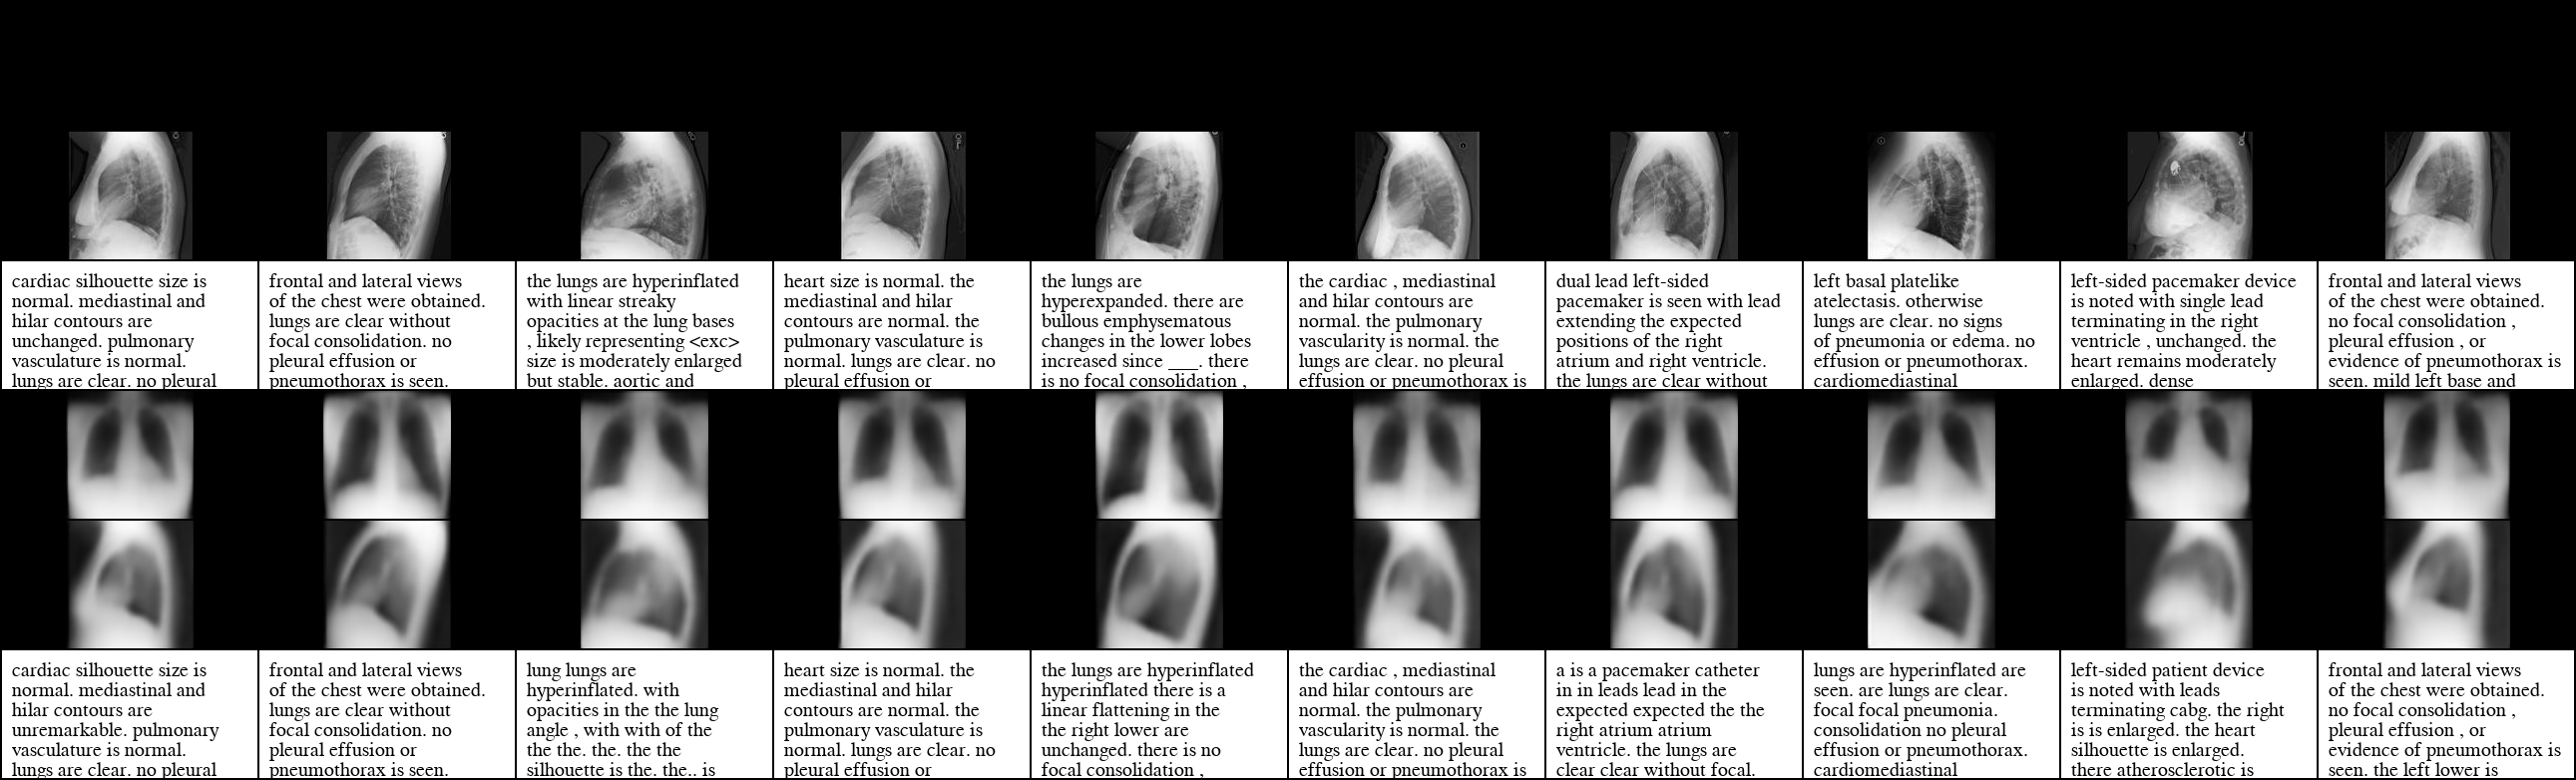
\includegraphics[width=\textwidth]{data/cond_gen/Lateral_text}
    \caption{
        \textbf{Conditionally generated samples with F and T modalities as conditioner.} The second and third image rows were given to the model as conditioner. The three last images rows are the generated samples. The images in the first row are the scans that correspond to the samples given as conditioner. The generated samples are blurry and it is difficult to see wether they represent some of the features that are characteristic to the input samples.
    }
    \label{fig:fig_cond_lattext}
\end{figure}

\begin{figure}
    \centering
    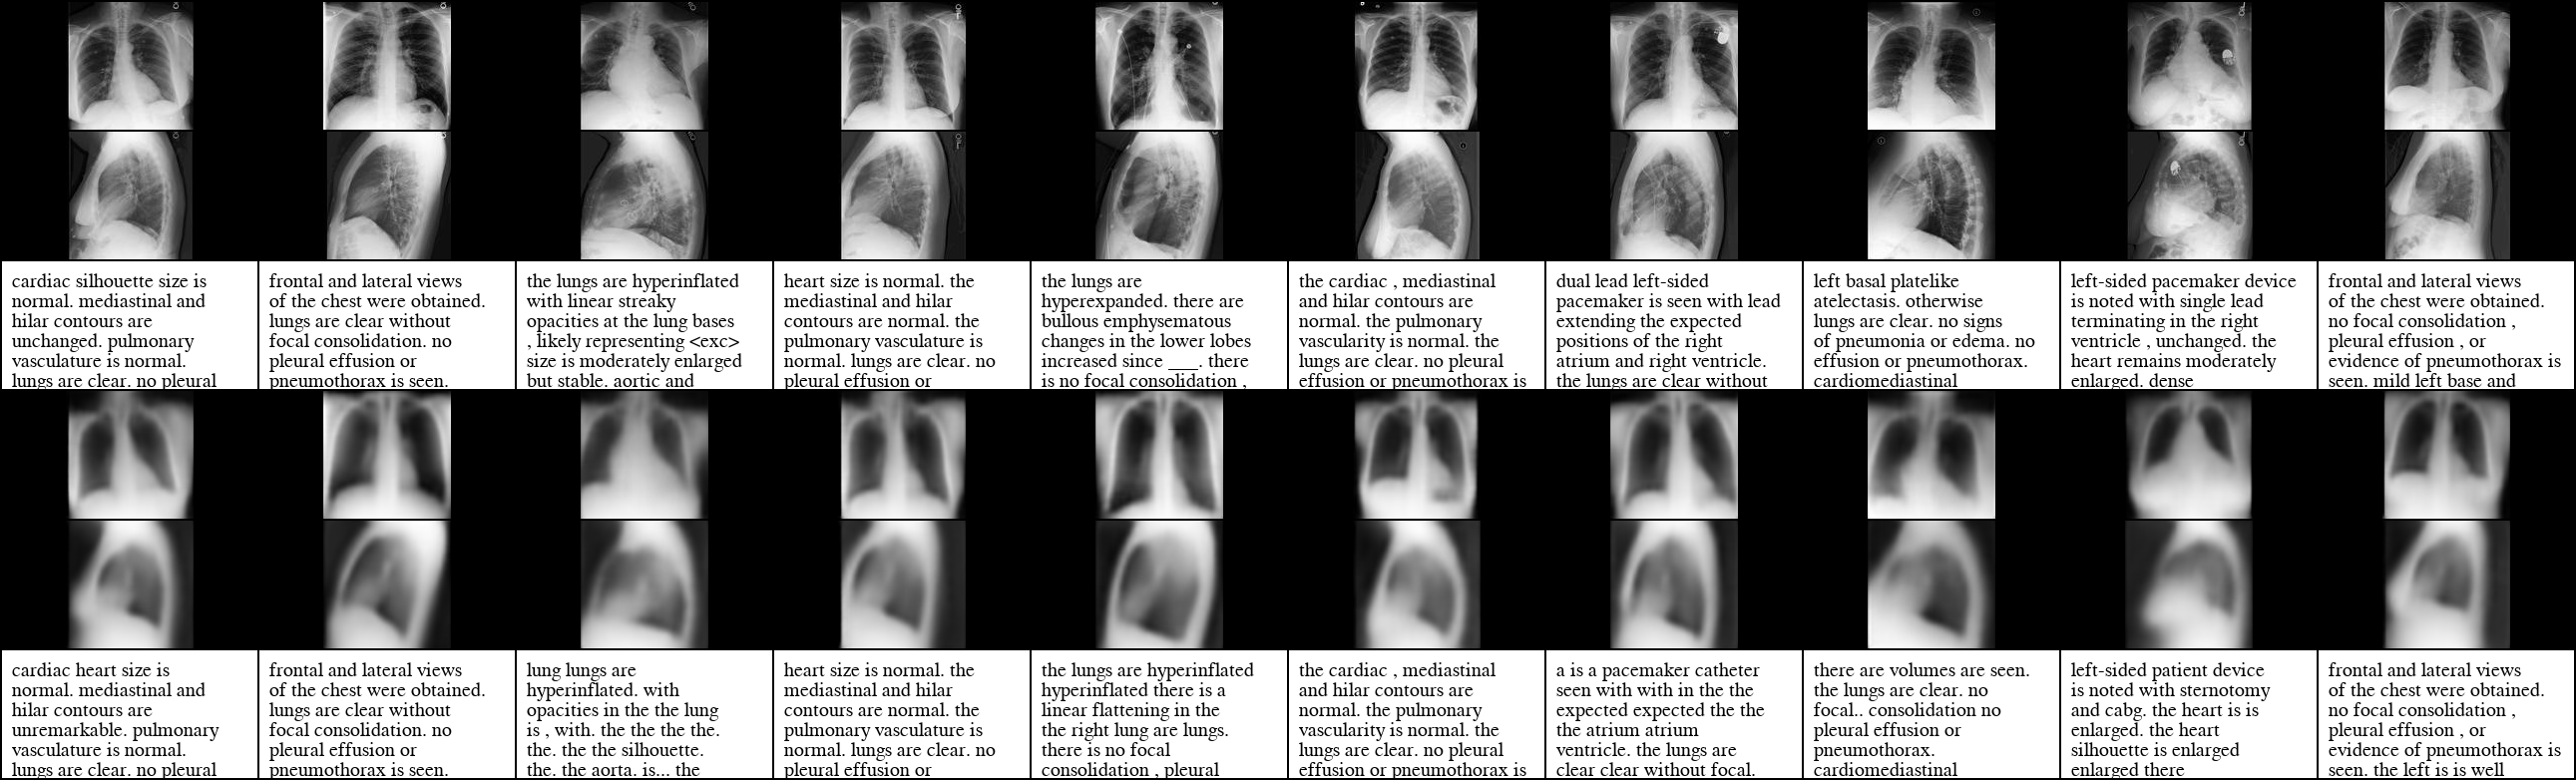
\includegraphics[width=\textwidth]{data/cond_gen/Lateral_PA_text}
    \caption{
        \textbf{Conditionally generated samples with F, L and T modalities as conditioner.} While the generated images are blurry, they do present some features that can be found in the input samples.
    }
    \label{fig:fig_cond_latPAtext}
\end{figure}


\py{
    pytex_tab(
    script='scripts/gen_eval_table.py',
    label='gen_eval_table',
    caption='\\textbf{Evaluation of the generation coherence.} For conditional generation, the letter below the horizontal line indicates the modality which is generated based on the input subsets $\\xset _k$ above. We report the mean average precision values between the prediction of a trained classifier on the generated samples and the label of the input samples.',
    options_pre='\\centering \\resizebox{0.9\\textwidth}{!}{',
    options_post='}',
    )
}
